\documentclass[a4paper]{article}
\usepackage[warn]{mathtext} %для поддержки кириллицы в формулах
\usepackage{amsmath} %основной пакет для формул
\usepackage[utf8x]{inputenc}
\usepackage[T1,T2A]{fontenc}
\usepackage[russian]{babel}
\usepackage{hyperref}
\usepackage{indentfirst}
\usepackage{listings}
\usepackage{color}
\usepackage{xcolor}
\usepackage{here}
\usepackage{array}
\usepackage{multirow}
\usepackage{graphicx}

\definecolor{linkcolor}{HTML}{000000} % цвет ссылок 000000 = чёрный
\definecolor{urlcolor}{HTML}{0000FF} % цвет гиперссылок 0000FF = синий
 
\hypersetup{pdfstartview=FitH, pagecolor=black, linkcolor=linkcolor,urlcolor=urlcolor, colorlinks=true}
\usepackage{caption}

\renewcommand{\lstlistingname}{Программа} % заголовок листингов кода

\usepackage{listings}
\lstset{ %
extendedchars=\true,
keepspaces=true,
language=c++,					% choose the language of the code
basicstyle=\footnotesize,		% the size of the fonts that are used for the code
numbers=left,					% where to put the line-numbers
numberstyle=\footnotesize,		% the size of the fonts that are used for the line-numbers
stepnumber=1,					% the step between two line-numbers. If it is 1 each line will be numbered
numbersep=5pt,					% how far the line-numbers are from the code
backgroundcolor=\color{white},	% choose the background color. You must add \usepackage{color}
showspaces=false				% show spaces adding particular underscores
showstringspaces=false,			% underline spaces within strings
showtabs=false,					% show tabs within strings adding particular underscores
frame=single,           		% adds a frame around the code
tabsize=2,						% sets default tabsize to 2 spaces
captionpos=b,					% sets the caption-position to bottom
breaklines=true,				% sets automatic line breaking
breakatwhitespace=false,		% sets if automatic breaks should only happen at whitespace
escapeinside={\%*}{*)},			% if you want to add a comment within your code
postbreak=\raisebox{0ex}[0ex][0ex]{\ensuremath{\color{red}\hookrightarrow\space}}
}

\usepackage[left=2cm,right=2cm,
top=2cm,bottom=2cm,bindingoffset=0cm]{geometry}

\newcommand{\RomanNumeralCaps}[1]
    {\MakeUppercase{\romannumeral #1}}


\begin{document}	% начало документа

\begin{titlepage}	% начало титульной страницы

	\begin{center}		% выравнивание по центру

		\large Санкт-Петербургский политехнический университет Петра Великого\\
		\large Институт компьютерных наук и технологий \\
		\large Кафедра компьютерных систем и программных технологий\\[2cm]
		% название института, затем отступ 6см
		
		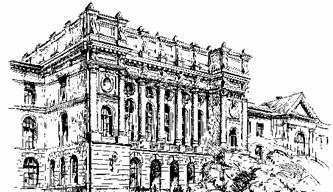
\includegraphics[scale=0.7]{pics/spbpu.jpg}\\[2cm]		
		
		\huge Курсовой проект по программированию\\
		\large Покер <<Техасский Холдем>>\\[8cm]
	\end{center}


	\begin{flushright} % выравнивание по правому краю
		\begin{minipage}{0.25\textwidth} % врезка в половину ширины текста
			\begin{flushleft} % выровнять её содержимое по левому краю

				\large\textbf{Работу выполнил:}\\
				\large Ламтев ~А.Ю.\\
				\large {Группа:} 13501/4\\
				
				\large \textbf{Преподаватель:}\\
				\large Вылегжанина ~К.Д.

			\end{flushleft}
		\end{minipage}
	\end{flushright}
	
	\vfill % заполнить всё доступное ниже пространство

	\begin{center}
	\large Санкт-Петербург\\
	\large \the\year % вывести дату
	\end{center} % закончить выравнивание по центру

\thispagestyle{empty} % не нумеровать страницу
\end{titlepage} % конец титульной страницы

\vfill % заполнить всё доступное ниже пространство



% Содержание
\hypertarget{toc}
\tableofcontents
\newpage

%TODO

\section*{Глава 1. Покер <<Техасский Холдем>>}
\addcontentsline{toc}{section}{Глава 1. Покер <<Техасский Холдем>>}

%Глава -- Описание предметной области (должно называться типа "Японская игра Сеги", "Эмулятор звездной системы", "Модель хищник-жертва" и %т. п.). Там размещаем то, что есть в ваших репозиториях в README.md, кроме диаграммы компонентов.\\

С древних времен люди любили играть в азартные игры, в том числе карточные и такие, как покер.

\subsection*{Задание}
\addcontentsline{toc}{subsection}{Задание}

  Разработать приложение на языке Java, реализующее игру Покер <<Техасский Холдем>>.

\subsection*{Правила игры}
\addcontentsline{toc}{subsection}{Правила игры}
	Правила были взяты с \texttt{сайта} Канцелярии генерального прокурора департамента юстиции штата Калифорния США. \footnote{https://oag.ca.gov/sites/all/files/agweb/pdfs/gambling/BGC\_texas.pdf}
 
\subsection*{Концепция}
\addcontentsline{toc}{subsection}{Концепция}

  Готовый программный продукт включает в себя десктоп приложение с графическим интерфейсом, позволяющее пользователю играть в Покер <<Техасский Холдем>> против "компьютера".

Расширением функциональности может быть создание веб-сервера и веб-приложения с возможностю игры нескольких пользователей в режиме online, android-приложение, а так же реализация других версий покера помимо <<Техасского Холдема>>, например, <<Омаха Холдем>>.

\subsection*{Минимально работоспособный продукт (Minimum Viable Product - MVP)}
\addcontentsline{toc}{subsection}{Минимально работоспособный продукт (Minimum Viable Product - MVP)}

 Графическое десктоп приложение, позволяющее играть нескольким пользователям с одного компьютера.

\subsection*{Вывод}
\addcontentsline{toc}{subsection}{Вывод}

Автор познакомился с предметной областью Покера <<Техасский Холдем>>, и решил, что реализация этой игры отлично подходит в качестве курсового проекта в рамках объектно-ориентированного программирования.

\section*{Глава 2. Проектирование приложения, реализующего игру Покер <<Техасский Холдем>>}
\addcontentsline{toc}{section}{Глава 2. Проектирование приложения, реализующего игру Покер <<Техасский Холдем>>}

%Глава -- Проектирование ("Проектирование приложения, реализующего эмулятор звездной системы/японскую игру сеги/модель хищник-жертва". %Здесь описываете архитектуру приложения -- сколько каких подпроектов (какие библиотеки, приложения, тесты), диаграмма компонентов, %описание выделенных интерфейсов (API) человеческим языком, дополнительных библиотек (если использовали), версии языка, кьюти, %компилятора. Описать структуру файлов, если какие-то создаются в процессе работы приложения.\\

В ходе проектирования было принято решение выделить 2 подпроекта: ядро - \textbf{core} и десктоп приложение с графическим интерфейсом - \textbf{desktop}. На рис. \ref{pic:component} изображена диаграмма компонентов проекта.

\begin{figure}[H]
	\begin{center}
		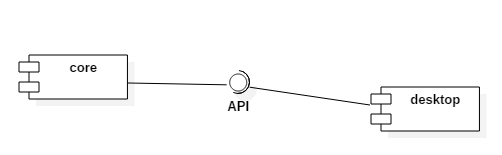
\includegraphics[scale=1]{pics/component_diagram.png}
	    \caption{Диаграмма компонентов} 
		\label{pic:component}
	\end{center}
\end{figure}


%TODO мб добавить описание диаграммы

\subsection*{core}
\addcontentsline{toc}{subsection}{core}

\textbf{core} - подпроект, в котором реализуется бизнес-логика Покера <<Техасский Холдем>>

\subsubsection*{Программный интерфейс приложения (Application Programming Interface - API)}
\addcontentsline{toc}{subsection}{Программный интерфейс приложения (Application Programming Interface - API)}

В подпроекте core был выделен пакет (Java package), в котором представлены классы API:



\subsection*{desktop}
\addcontentsline{toc}{subsection}{desktop}

Подпроект desktop - десктоп приложение с графическим интерфейсом.

\subsection*{Вывод}
\addcontentsline{toc}{subsection}{Вывод}

В ходе проектирования было принято решение, каким образом делить на подпроекты, какие компонетны выделить и какие методы интерфейсов определить.

\section*{Глава 3. Реализация игры Покер <<Техасский Холдем>>}
\addcontentsline{toc}{section}{Глава 3. Реализация игры Покер <<Техасский Холдем>>}

%Глава -- Реализация ("Реализация японской игры сеги/модели хищник-жертва"). Здесь описываете среду разработки (версии всех использованых %ос, компиляторов, сред, утилит (qt creator, doxygen, прочее)), очень поверхностно описываете, какие основные классы выделили в каждом из %проектов, если какие-то интересные паттерны или алгоритмы -- тоже. Можно тут рассказать, сколько строк кода. Приводите скрины основных %%экранов пользовательского интерфейса, но чтоб не только картинки, но еще и слова, описывающие то, что видно на картинке. К картинкам не %забывайте делать подписи.

\subsection*{Среда разработки}
\addcontentsline{toc}{subsection}{Среда разработки}

\noindent\textbf{Операционная система:} Windows 10.0.10586\\
\textbf{Интегрированная среда разработки:} JetBrains IntelliJ IDEA 2016.2.3 - 2016.3.1\\
\textbf{Уровень языка Java:} java 8 standart edition\\
\textbf{Компилятор:} jdk 1.8.0\_112\\
\textbf{Фреймворк для GUI:} JavaFX8\\
\textbf{Система автоматизации сборки:} Gradle 3.0 - 3.2.1\\
\textbf{Система контроля версий:} Git 2.9.2\\

\subsection*{core}
\addcontentsline{toc}{subsection}{core}

Было выделено 48 классов, содержащих функциональность ядра.

\textbf{Классы:}

\begin{itemize}

\item api

\begin{enumerate}

\item CardDeck
\item CommunityCardsListener
\item CurrentPlayerListener
\item GameIsOverListener
\item MoveAbilityListener
\item PlayerExpandedInfo
\item PlayerFoldListener
\item PlayerInfo
\item PlayerMoney
\item PlayerShowedDownListener
\item Poker
\item PokerAPI
\item PreflopMadeListener
\item StateChangedListener
\item WagerPlacedListener

\end{enumerate}

\item model

\begin{enumerate}

\item Bank
\item Card
\item CardDeck
\item Cards
\item Dealer
\item Player
\item Players
\item Rank
\item Suit

\end{enumerate}

\item hands

\begin{enumerate}

\item Flush
\item  FourOfAKind
\item  FullHouse
\item  HighCard
\item  Pair
\item  PokerHand
\item  PokerHandFactory
\item  RoyalFlush
\item  Straight
\item StraightFlush
\item ThreeOfAKind
\item TwoPairs

\end{enumerate}

\item states

\begin{enumerate}

\item GameIsOverException
\item GameHaveNotBeenStartedException
\item ActionPokerState
\item FlopWageringPokerState
\item GameIsOverPokerState
\item MoveValidator
\item PokerState
\item PreflopWageringPokerState
\item RiverWageringPokerState
\item SettingsPokerState
\item ShowdownPokerState
\item TurnWageringPokerState
\item WageringPokerState

\end{enumerate}

\end{itemize}

На рис. \ref{pic:core:1} изображена диаграмма классов ядра.


\begin{figure}[H]
	\begin{center}
		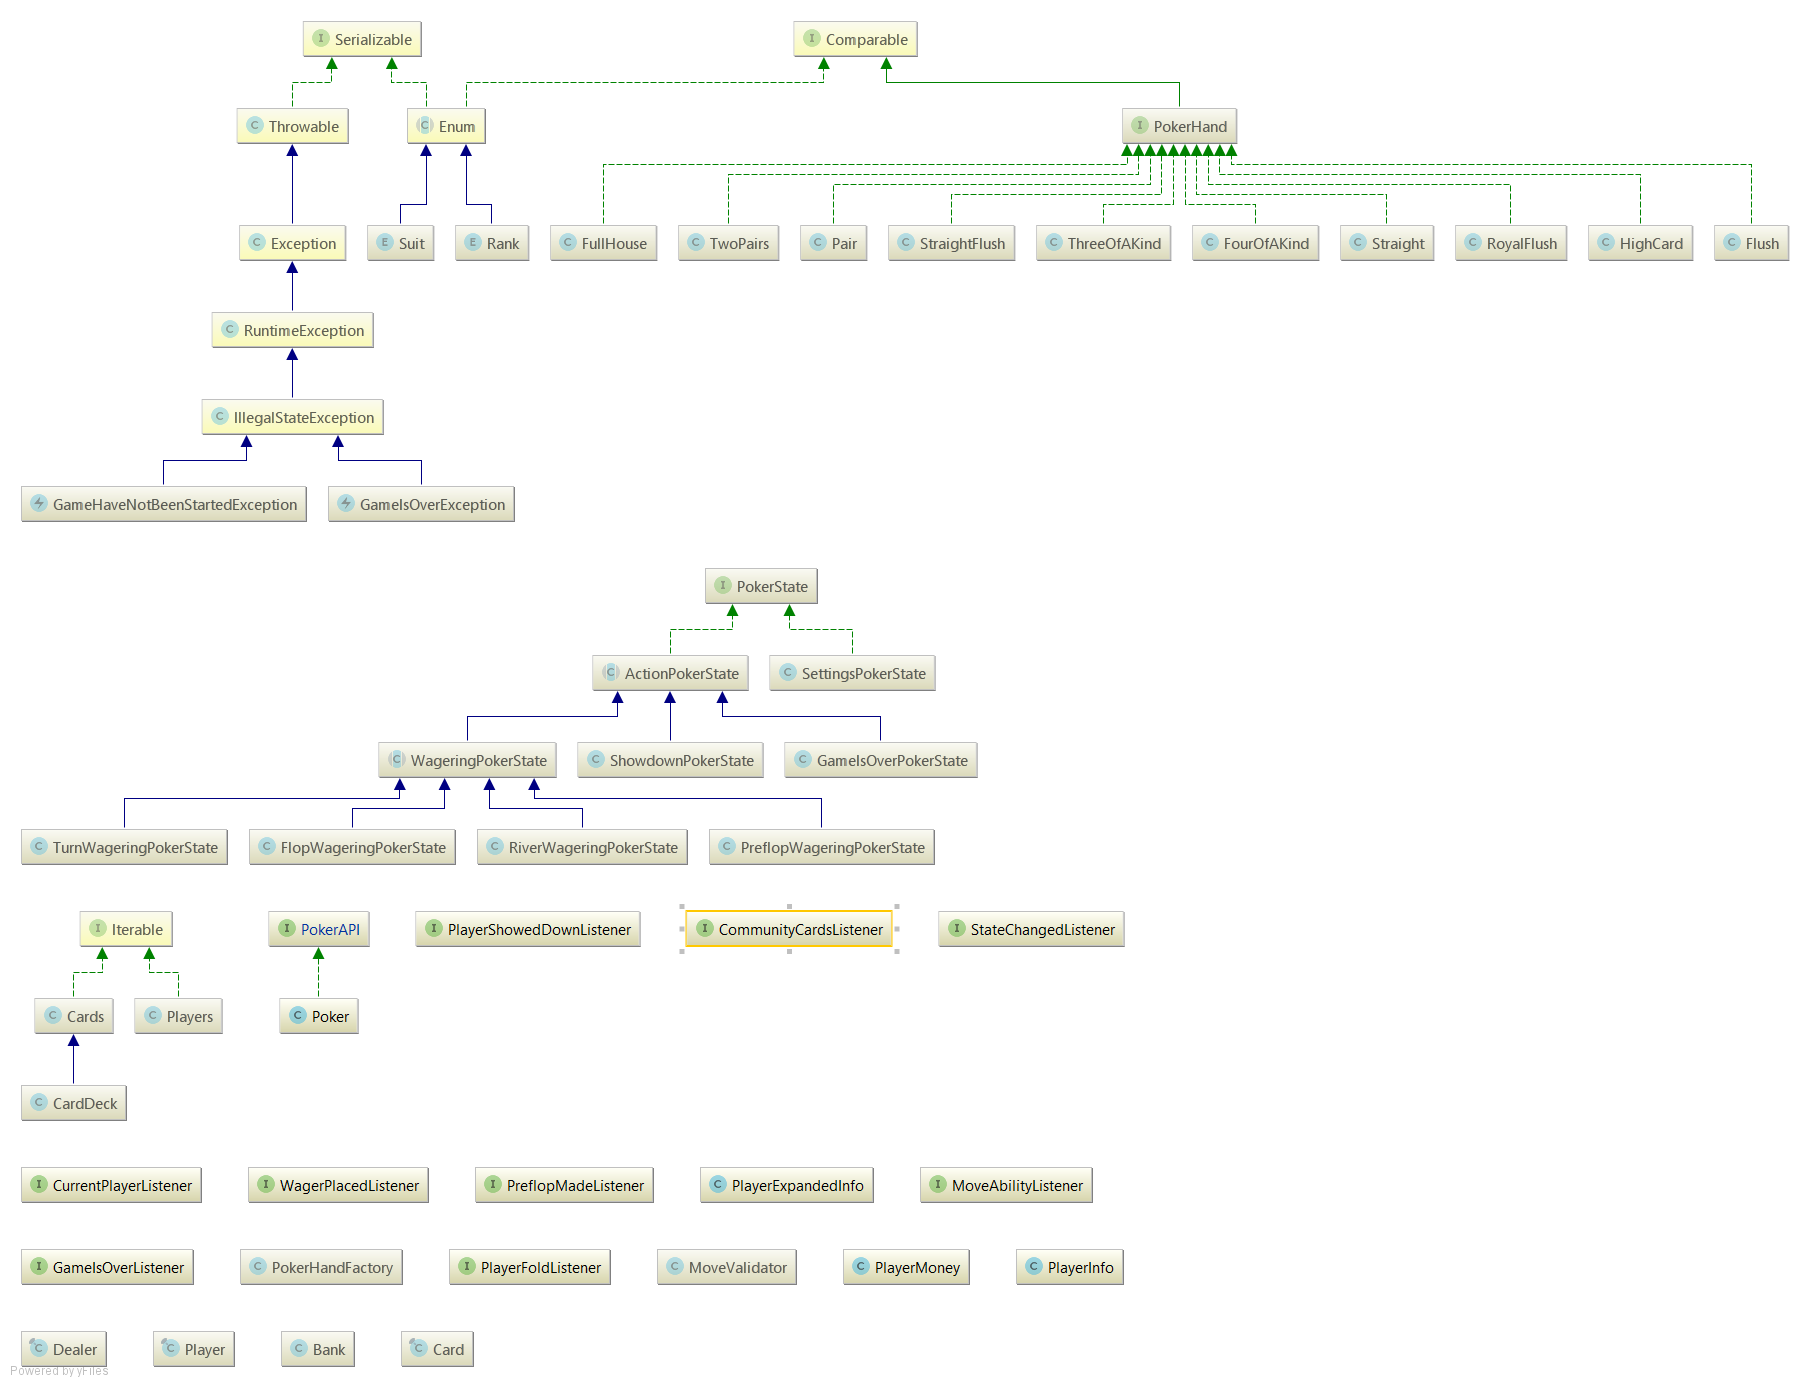
\includegraphics[scale=0.28]{pics/class_diagram.png}
	    \caption{Диаграмма классов} 
		\label{pic:core:1}
	\end{center}
\end{figure}

\subsection*{desktop}
\addcontentsline{toc}{subsection}{desktop}

Графическое приложение было разработано с использование фреймворка JavaFX8. Оно помимо взаимодействия с пользователем содержит еще и простой искусственный интеллект, что позволяет играть пользователю против "компьютера".

На рисунках ниже представлены снимки экрана с запущенным приложением.

\begin{figure}[H]
	\begin{center}
		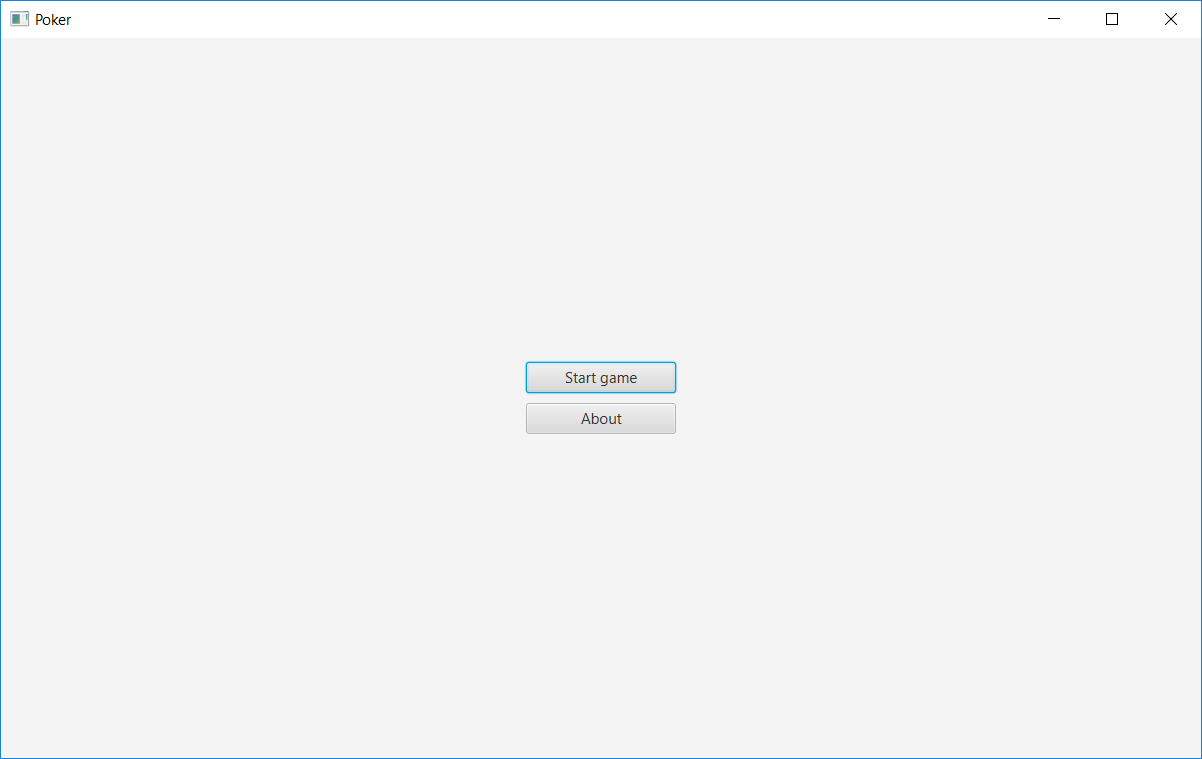
\includegraphics[scale=0.5]{pics/1.png}
	    \caption{Начальный экран} 
		\label{pic:gui:1}
	\end{center}
\end{figure}

\begin{figure}[H]
	\begin{center}
		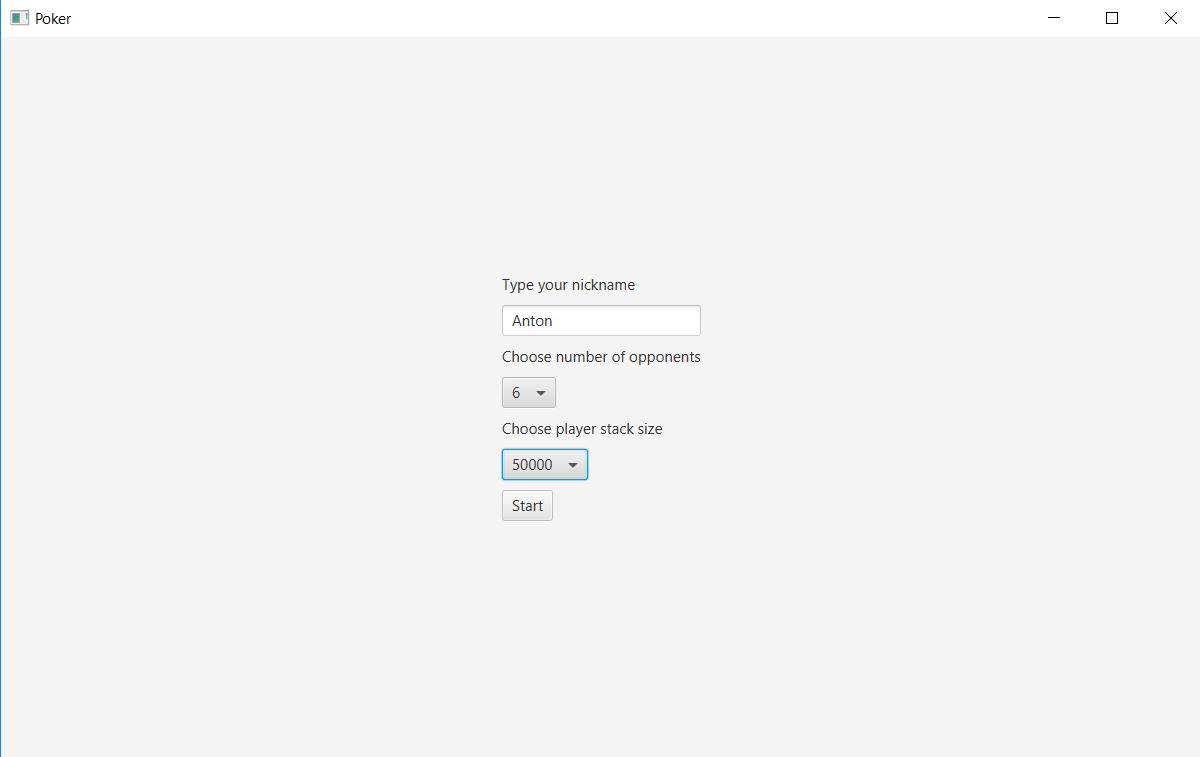
\includegraphics[scale=0.5]{pics/2.png}
	    \caption{Предыгровые настройки} 
		\label{pic:gui:2}
	\end{center}
\end{figure}

\begin{figure}[H]
	\begin{center}
		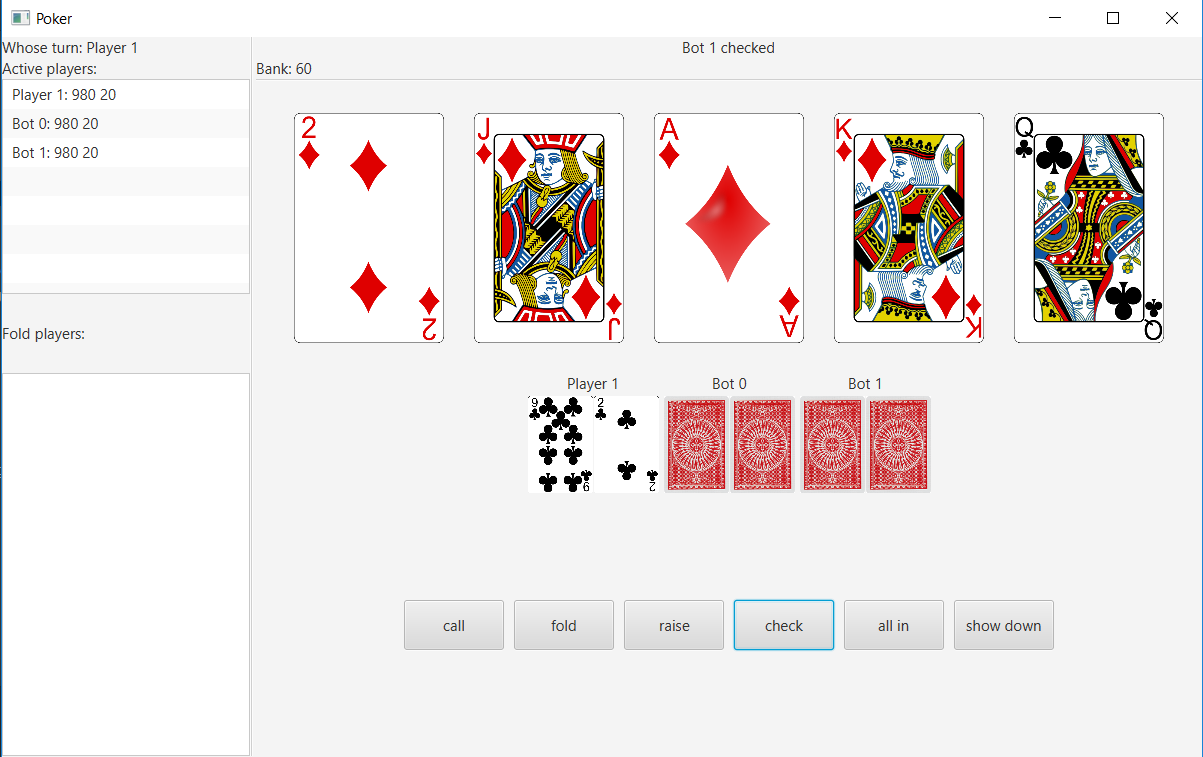
\includegraphics[scale=0.5]{pics/3.png}
	    \caption{Игровой процесс} 
		\label{pic:gui:3}
	\end{center}
\end{figure}

\begin{figure}[H]
	\begin{center}
		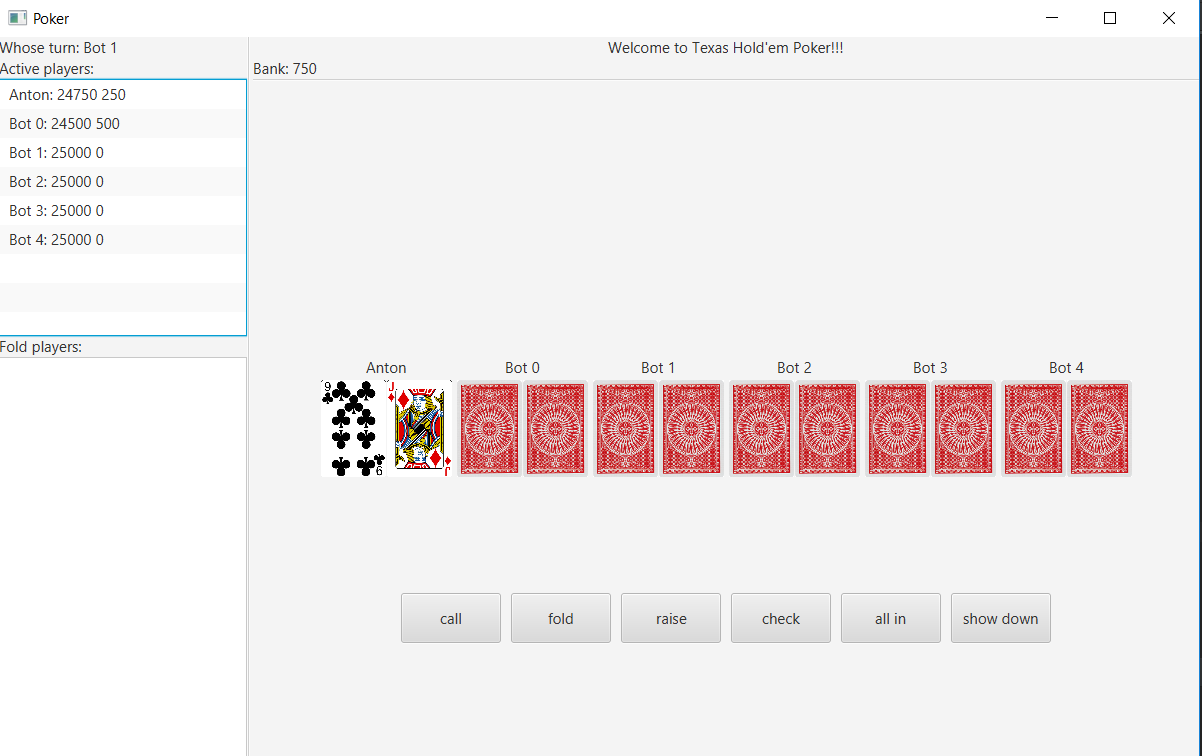
\includegraphics[scale=0.5]{pics/4.png}
	    \caption{Игровой процесс} 
		\label{pic:gui:4}
	\end{center}
\end{figure}

\begin{figure}[H]
	\begin{center}
		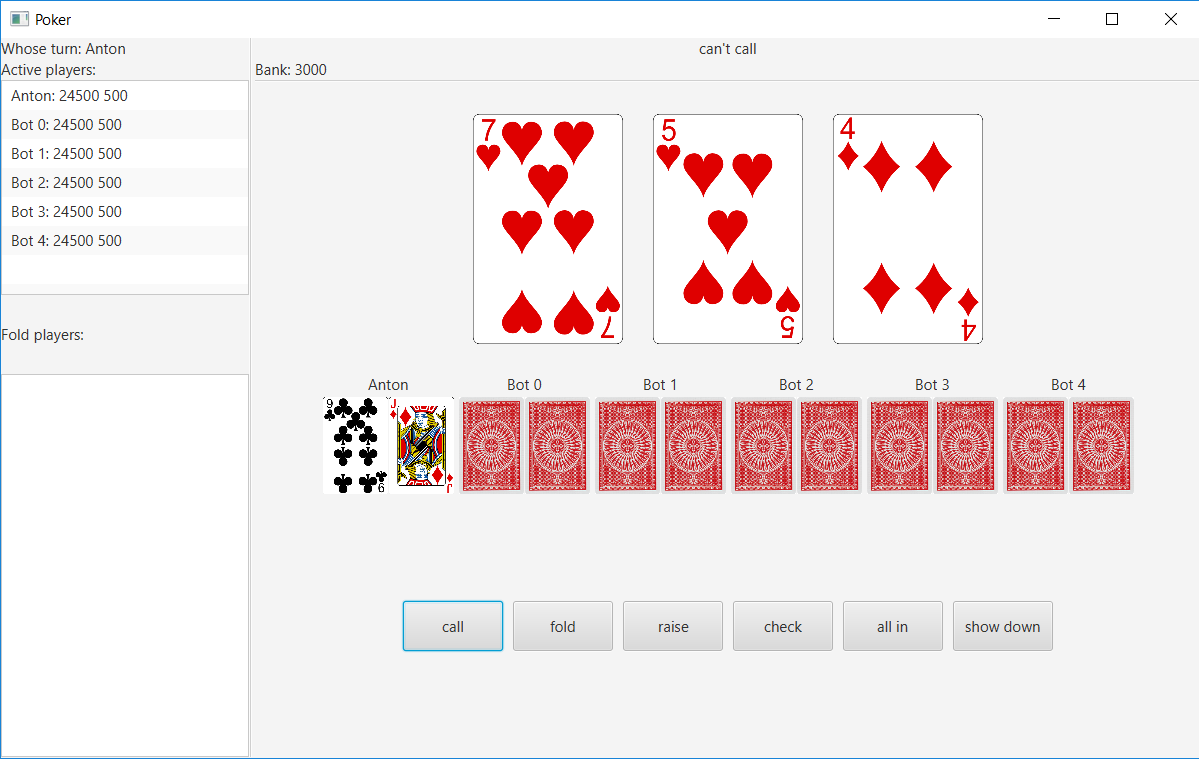
\includegraphics[scale=0.5]{pics/5.png}
	    \caption{Диаграмма компонентов} 
		\label{pic:gui:5}
	\end{center}
\end{figure}

\begin{figure}[H]
	\begin{center}
		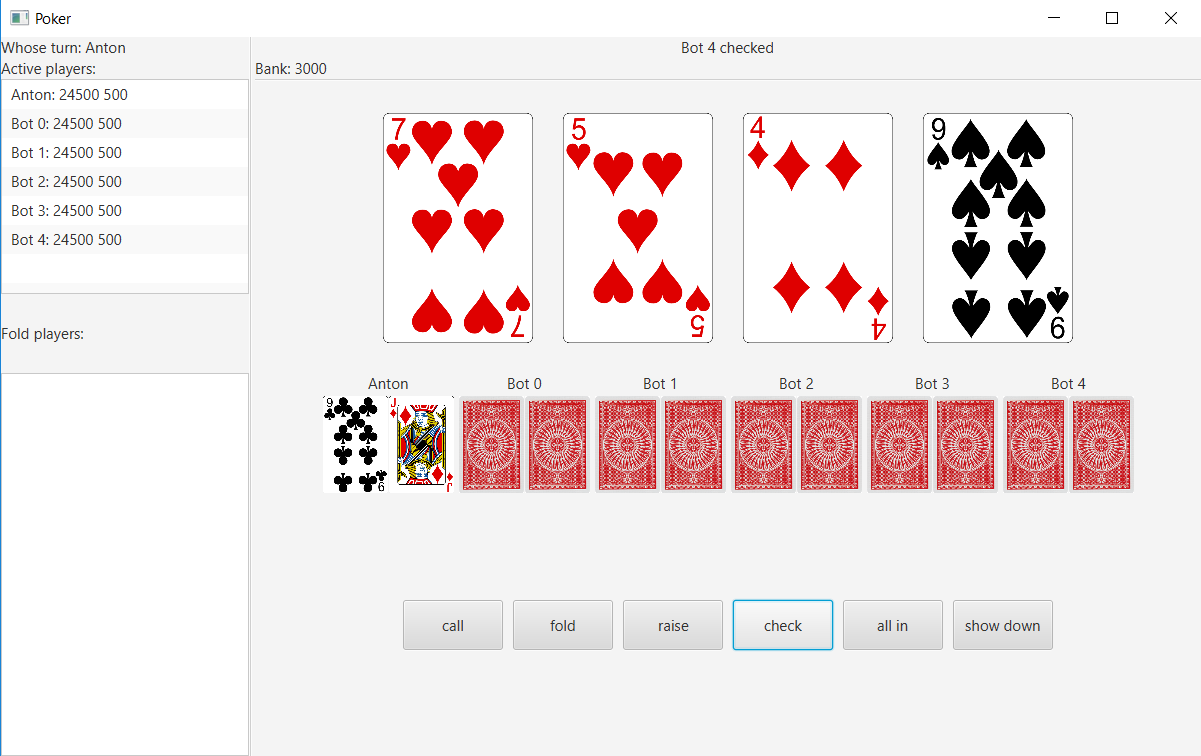
\includegraphics[scale=0.5]{pics/6.png}
	    \caption{Игровой процесс} 
		\label{pic:gui:6}
	\end{center}
\end{figure}

\begin{figure}[H]
	\begin{center}
		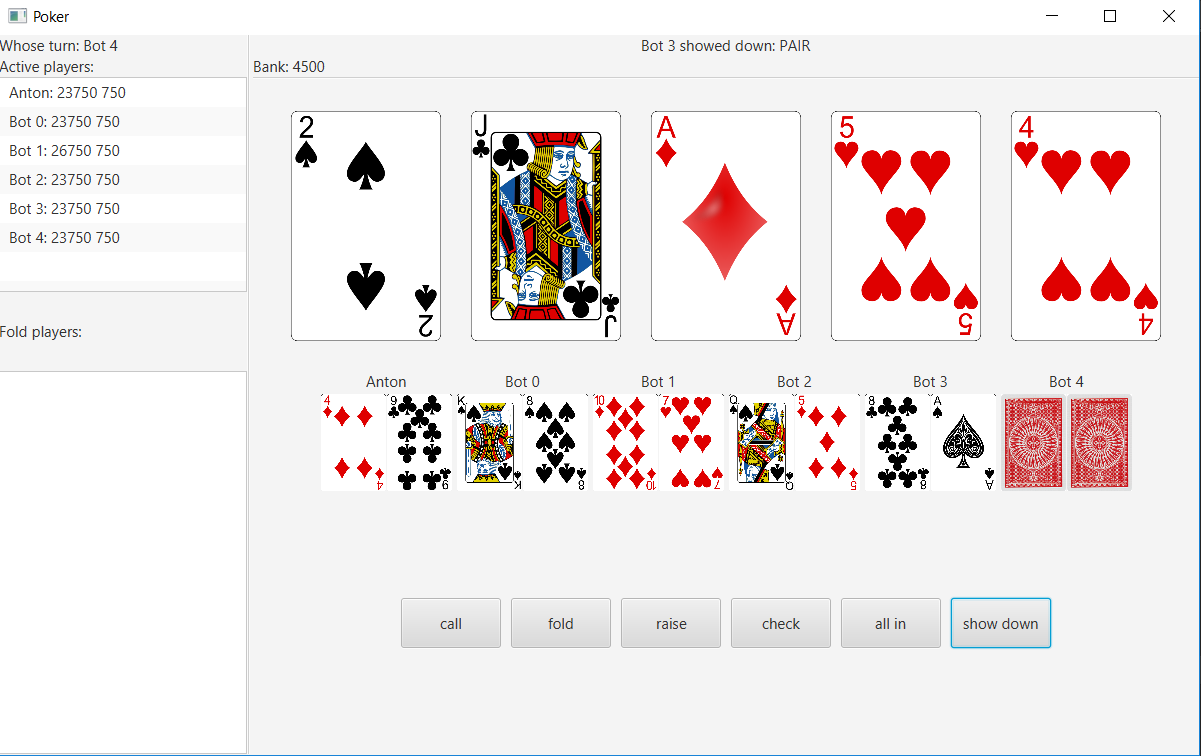
\includegraphics[scale=0.5]{pics/7.png}
	    \caption{Игровой процесс: Пара} 
		\label{pic:gui:6}
	\end{center}
\end{figure}

\begin{figure}[H]
	\begin{center}
		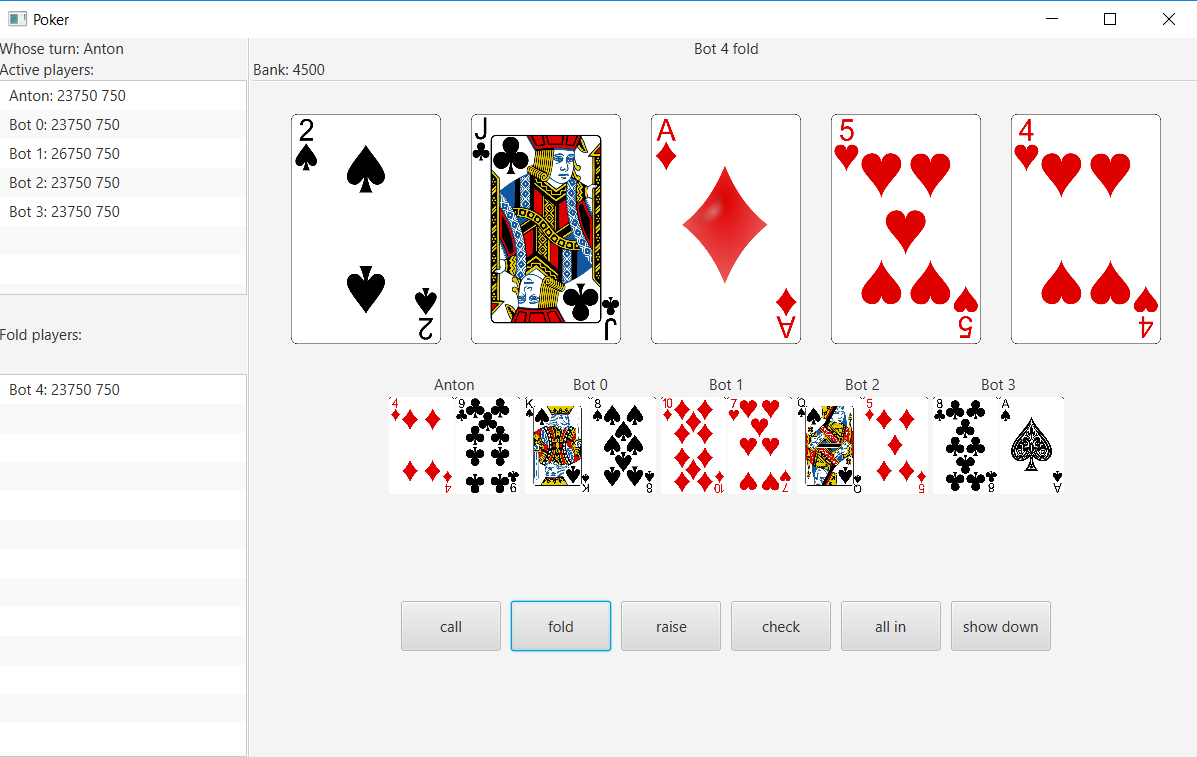
\includegraphics[scale=0.5]{pics/8.png}
	    \caption{Игровой процесс} 
		\label{pic:gui:6}
	\end{center}
\end{figure}

\begin{figure}[H]
	\begin{center}
		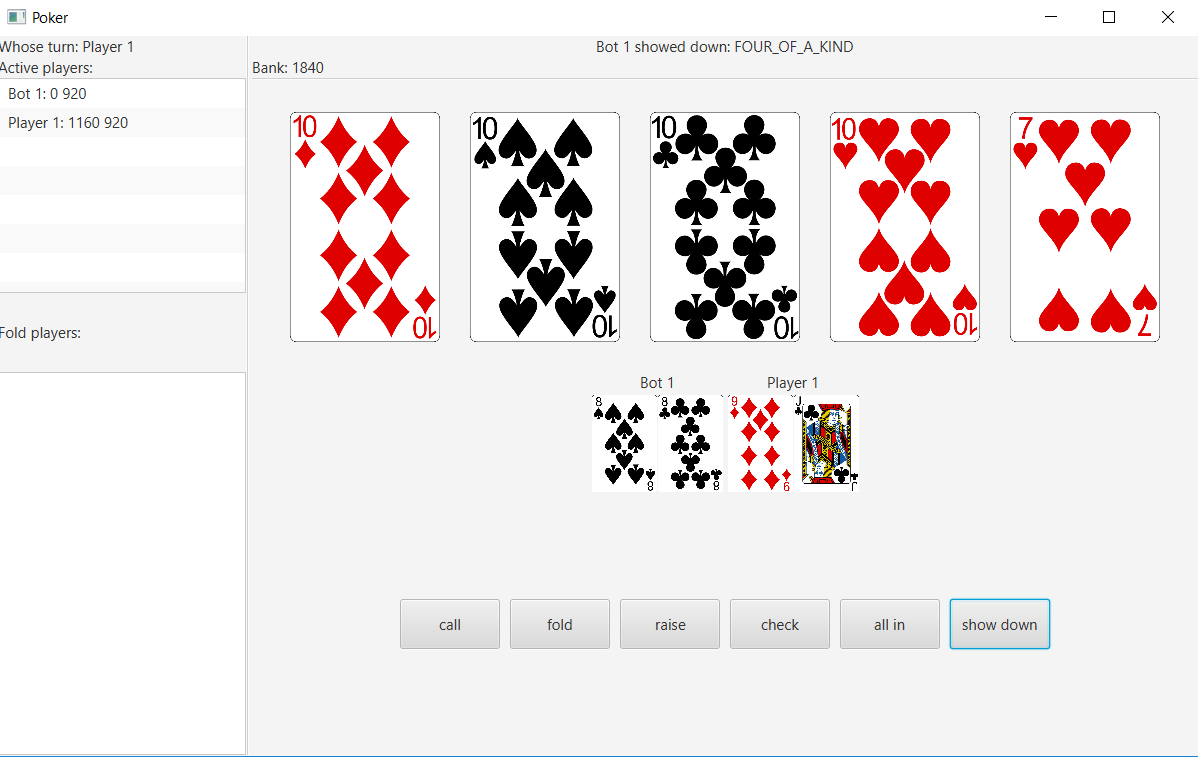
\includegraphics[scale=0.5]{pics/9.png}
	    \caption{Игровой процесс: Каре} 
		\label{pic:gui:6}
	\end{center}
\end{figure}

\begin{figure}[H]
	\begin{center}
		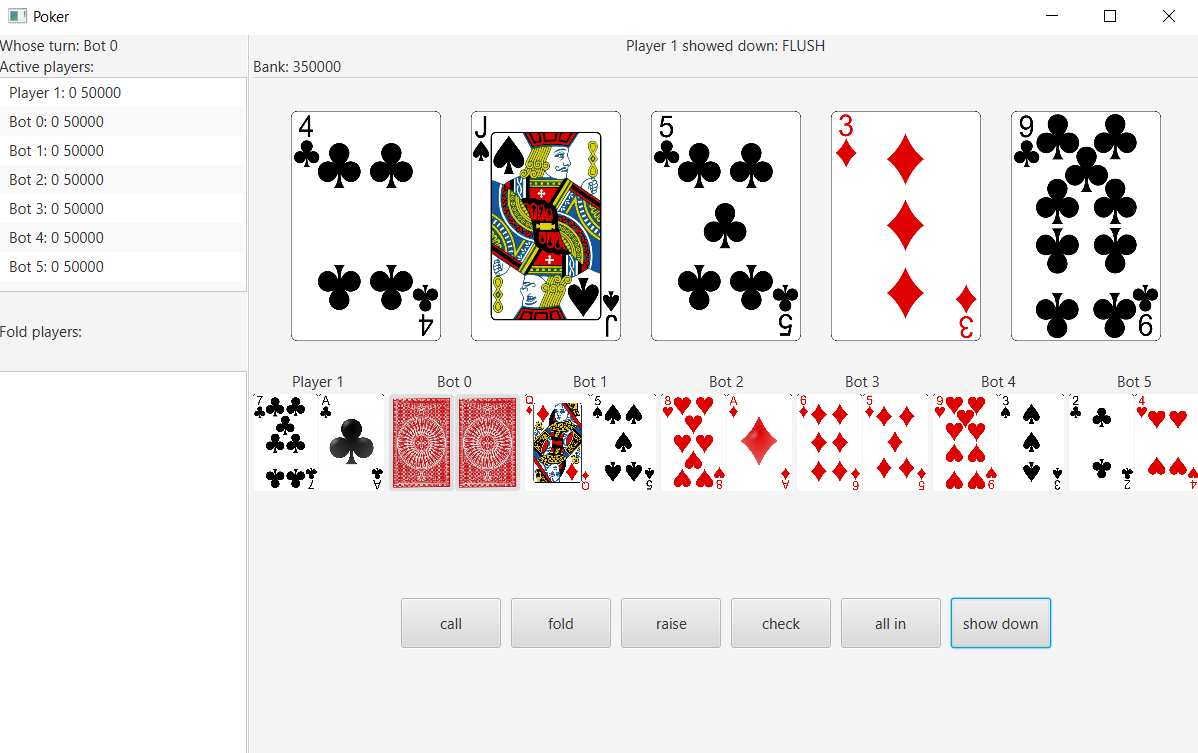
\includegraphics[scale=0.5]{pics/10.png}
	    \caption{Игровой процесс: Флеш} 
		\label{pic:gui:6}
	\end{center}
\end{figure}

\subsection*{Вывод}
\addcontentsline{toc}{subsection}{Вывод}

В ходе разработки приложения автор получил большой опыт в объектно-ориентированном программировании на языке java. 
Были применены паттерны объектно-ориентированного программирования <<Банды четырех>> (Gang of foor) \footnote{https://ru.wikipedia.org/wiki/Design\_Patterns}: Наблюдатель, Состояние, Абстрактная фабрика. Автором были освоены различные возможности языка java версии 8, такие как: lambdas, stream api.

\section*{Глава 4. Процесс обеспечения качества и тестирование}
\addcontentsline{toc}{section}{Глава 4. Процесс обеспечения качества и тестирование}

%Глава -- "Процесс обеспечения качества и тестирование". Здесь описываете процесс разработки -- количество ревью (и примерное количество %замечаний), количество демонстраций (с указанием конкретных замечаний и комментариями по ним), список использованных утилит (cppcheck, %valgrind, gcov и т.д, кто пользовался jenkins -- про него тоже) с комментариями как и когда они помогали. Рассказать про автоматические %тесты (модульные, функциональные), про тестовые сценарии, которые они покрывают, процент покрытия. Рассказать про тестовые сценарии для %ручных тестов.

Разработка велась в цикле непрерывной интеграции (continuous integration - ci). Кроме того, она сопровождалась ручным и автоматическим(модульным и функциональным) тестированием, статическим анализом кода, просмотрами кода (code review).

\subsection*{Тестирование}
\addcontentsline{toc}{subsection}{Тестирование}

\subsubsection*{Автоматическое тестирование}
\addcontentsline{toc}{subsubsection}{Автоматическое тестирование}

Частично разработка велась согласно подходу TDD (Test-Driven Development), когда сначала сразу после проектирования интерфейса класса пишутся модульные тесты, а затем реализуется функциональность класса. Все классы, которые получилось протестировать модульными тестами, были протестированы модульными тестами. Затем, когда независимые и протестированные модули начали взаимодействовать друг с другом, появилась необходимость в функциональных тестах.

Для автоматического тестирования использовался фреймворк JUnit 4.12.

Для удобного отображения результатов подсчета покрытия тестами кода использовался сервис Codecov \footnote{https://codecov.io}

 На рис. ref{pic:test:1} видно, что покрытие автоматическими тестами строчек кода ядра составляет 73\% ,что является хорошим результатом. Очень многие баги были найдены еще на этапе автоматического тестирования.

\begin{figure}[H]
	\begin{center}
		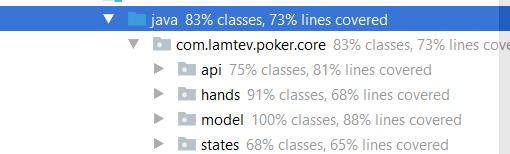
\includegraphics[scale=0.5]{pics/coverage.png}
	    \caption{Процент покрытия} 
		\label{pic:test:1}
	\end{center}
\end{figure}

\subsubsection*{Ручное тестирование}
\addcontentsline{toc}{subsubsection}{Ручное тестирование}

Ручное тестирование было.

\subsection*{Статический анализ}
\addcontentsline{toc}{subsubsection}{Статический анализ}

Статический анализ проводился при помощи JetBrains IntelliJ IDEA inspections и find-bugs. Все найденные ими недочеты в коде были исправленны.

\subsection*{Непрерывная интеграция}
\addcontentsline{toc}{subsection}{Непрерывная интеграция}

Непрерывная интеграция осуществлялась с помощью платформы Travic-ci.\footnote{https://travis-ci.org}
	
В цикле ci внутри cобственного \textbf{docker} контейнера \textbf{lamtev/java}\footnote{https://hub.docker.com/r/lamtev/java/} запускались автоматические тесты, код анализировался статическим анализатором, велся подсчёт строк (утилита cloc 1.60).

На рис \ref{pic:travis:1} - \ref{pic:travis:3} приведены снимки экрана, демонстрирующие использование Travis-ci.

\begin{figure}[H]
	\begin{center}
		
\includegraphics[scale=0.75]{pics/travis1.png}
	    \caption{Travis-ci} 
		\label{pic:travis:1}
	\end{center}
\end{figure}

\begin{figure}[H]
	\begin{center}
		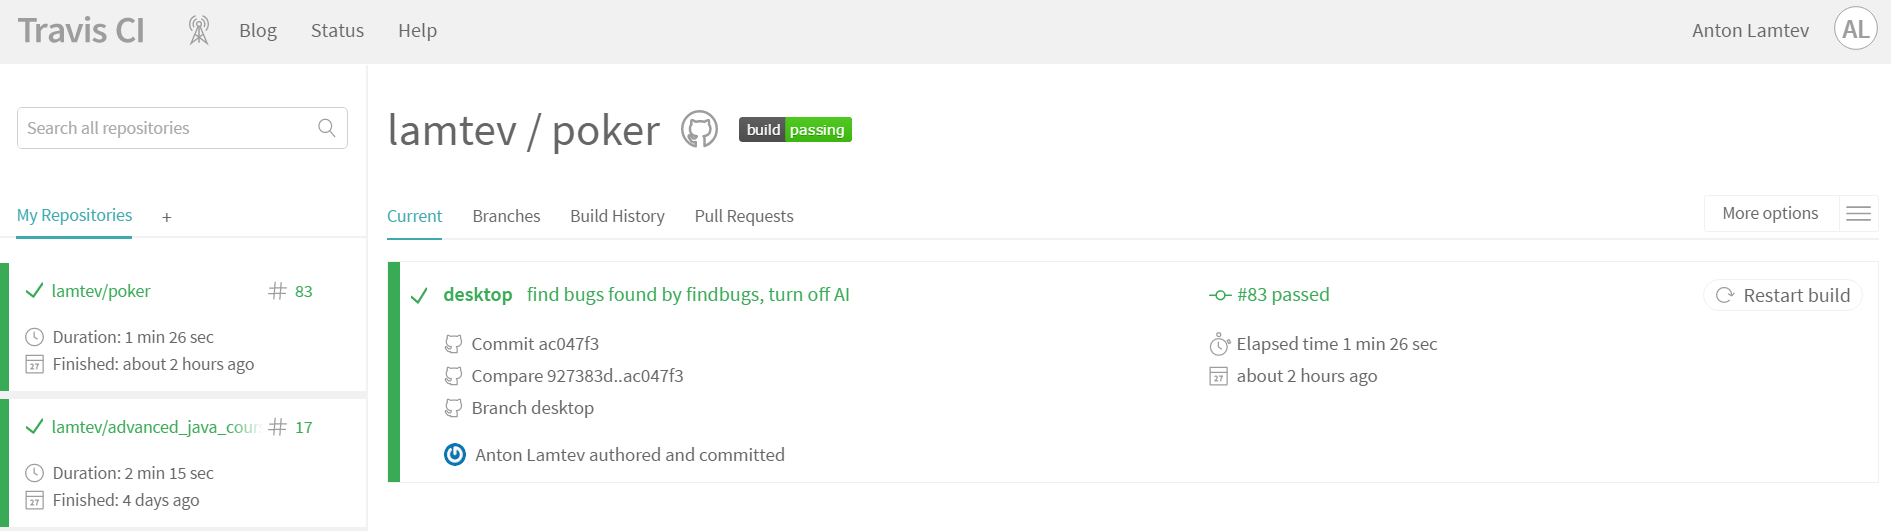
\includegraphics[scale=0.5]{pics/travis2.png}
	    \caption{Travis-ci} 
		\label{pic:travis:2}
	\end{center}
\end{figure}

На рис. \ref{pic:travis:3} приведен снимок экрана, на котором показано, что проект содержит 3406 строк кода на java

\begin{figure}[H]
	\begin{center}
		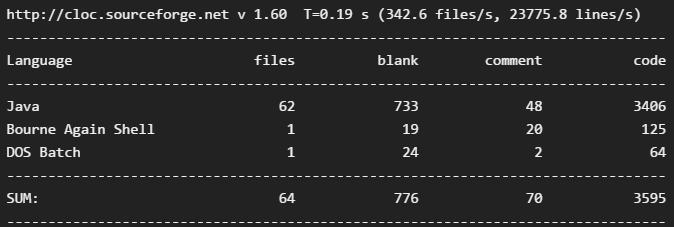
\includegraphics[scale=0.75]{pics/travis3.png}
	    \caption{Travis-ci: cloc} 
		\label{pic:travis:3}
	\end{center}
\end{figure}

\subsection*{Просмотр кода (Code Review)}
\addcontentsline{toc}{subsection}{Просмотр кода (Code Review)}

Автор в ходе разработки просил своих коллег: Дьячкова Вадима Вадимовича и Вылегжанину Карину Дмитриевну посмотреть его код. После их советов и указаний на недочеты в коде, были внесены правки. После одного из code review было принято решение использовать дизайн паттерны (Gang of four) Наблюдатель и Состояние.

\subsection*{Вывод}
\addcontentsline{toc}{subsection}{Вывод}

В ходе процесса обеспечения качества и тестирования автор получил навык написания кода, который легко тестировать. Автор получил опыт от использования непрерывной интеграции. Был получен опыт улучшения качества кода после code review от коллег.

\section*{Глава 5. Выводы}
\addcontentsline{toc}{section}{Глава 5. Выводы}

%своими словами, с душой, от чистого сердца рассказать, чему удалось научиться за семестр, что извлечь.
За семестр были получены первые навыки объекто-ориентированного проектирования и программирования приложений на языке java, а именно стандарте языка java 8. Автором были рассмотрены паттерны проектирования (Gang of four). 

В итоге получилось разбработать минимально работоспособный продукт.

Итак, автора продолжит разработку данного приложения в соответствии с концепцией.


\end{document}
